\documentclass[a4paper,12pt]{article}
\usepackage[portuguese]{babel}
\usepackage{graphicx}
%\graphicspath{ {/home/jessica/Documentos/Engineer/Geocaching-Java} }
\RequirePackage[T1]{fontenc}
\RequirePackage[utf8]{inputenc}

\renewcommand{\baselinestretch}{2}
%\author{no realizado por :P}
\title{Geocaching POO}
\date{Junho 2015}
\begin{document}
\maketitle
\begin{center}
Realizado por: \\
Jéssica Pereira a71164	\\

\includegraphics[height=3\baselineskip,natwidth=369,natheight=430]{jessica0.jpg}\\
Adelino Costa a70563\\
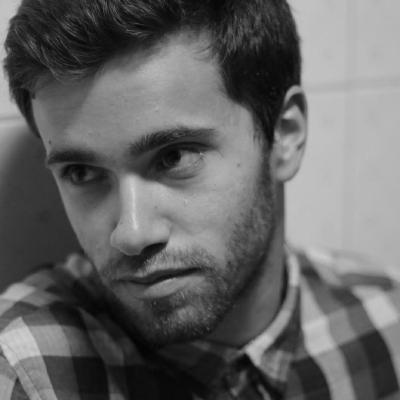
\includegraphics[height=3\baselineskip,natwidth=369,natheight=430]{adelino.jpg}\\
Martinho Aragão a72205 \\

\includegraphics[height=3\baselineskip,natwidth=369,natheight=430]{martinho.jpg}
\end{center}

\pagebreak


\tableofcontents

\pagebreak

\section{Introdução}
Este trabalho é sobre o conceito de Geocaching conhecido nas redes sociais: pretendemos simular e registar atividades e descobrimentos de caches. Para isso é necessário a modularizar  

Os objetivos são

Está organizado 

Metodologia utilizada

\section{Conclusão}


\section{}
\subsection{}
\subsubsection{}

\paragraph{paragraph title here}


\end{document}